\section{Back-propagation}

Il metodo di propagazione all'indietro dell'errore è applicabile a reti neurali
con un numero qualsiasi di strati di connessioni e con architetture molto
diverse. Proprio come la regola delta, modifica i pesi sinaptici in base alla
discrepanza tra la risposta fornita dalla rete e la risposta corretta.

\subsection{Algoritmo}

\begin{figure}[H]
	\centering
	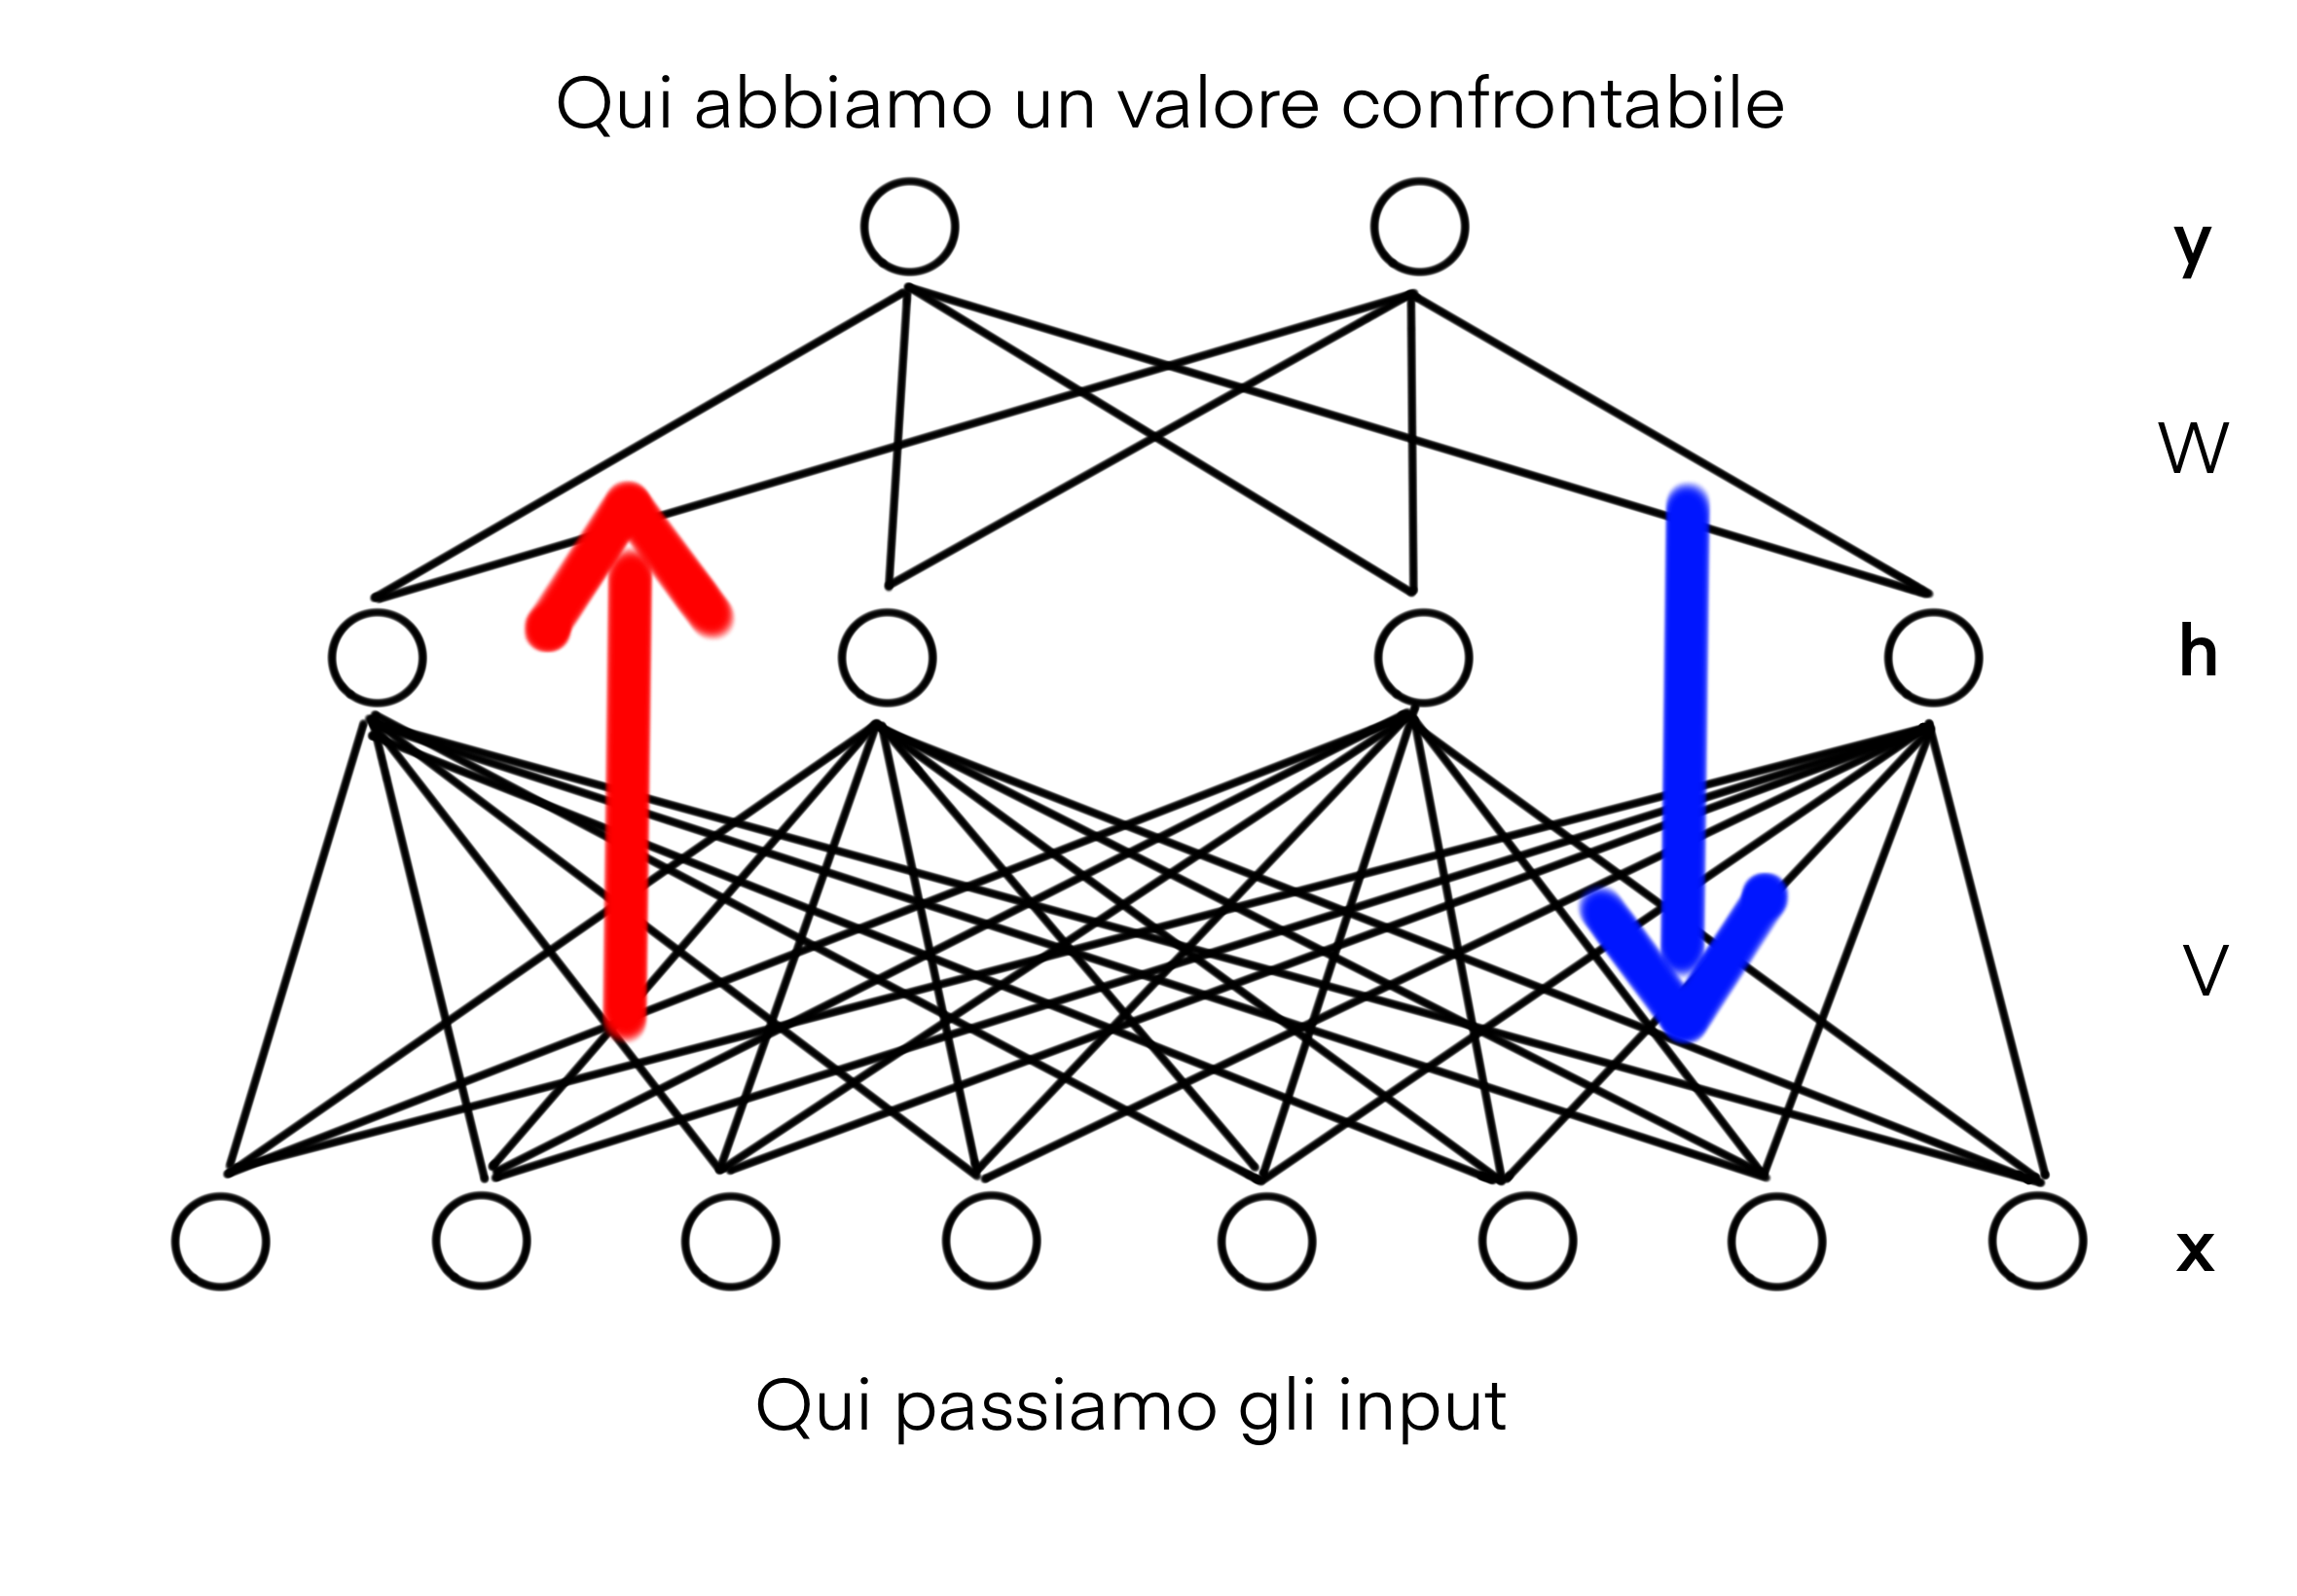
\includegraphics[width=0.5\textwidth]{backpropagation}
	\caption{Algoritmo di back-propagation, la freccia rossa indica il flusso
		del calcolo della previsione, mentre la freccia blu indica il flusso del
		calcolo dell'errore.}
	\label{fig:backpropagation}
\end{figure}

Consideriamo una rete feedfoward a due strati di connessioni con unità di input
$x_k$, unità interne $h_j$ e unità di output $y_i$. Indichiamo con $t^\mu_i$ il
valore della risposta correttà per ogni unità di output $i$ sull'input $\mu$.\\
Nell'esempio in questione, dunque abbiamo due strati di connessioni che devono
essere aggiornati. Spieghiamo i passi dell'algoritmo:

\begin{enumerate}
	\item \textbf{Input}: abbiamo in input un pattern d'ingresso $x$;

	\item \textbf{Forward pass 1}: calcoliamo l'attivazione di tutte le unità
	      interne $h_j = \phi(\sum_{k} v_{jk} x_k)$, dove $v_{jk}$ è il
	      peso della connessione tra l'unità in input $k$ e l'unità interna $j$;

	\item \textbf{Forward pass 2}: calcoliamo l'attivazione di tutte le unità di
	      output $y_i = \phi(\sum_{j} w_{ij} h_j)$, dove $w_{ij}$ è il peso
	      della connessione tra l'unità interna $j$ e l'unità di output $i$;

	\item \textbf{Calcolo dell'errore 1}: ora vogliamo minimizzare l'errore, quindi
	      confrontiamo il risultato ottenuto con il risultato corretto. Calcoliamo
	      la correzione dei pesi sinaptici come
	      \begin{equation*}
		      \Delta w_{ij} = \eta (t_i - y_i) \phi'(A_i) h_j,
	      \end{equation*}
	      dove $\eta$ è il tasso di apprendimento, $t_i$ è il
	      valore corretto dell'unità di output $i$, $y_i$ è il valore ottenuto
	      dall'unità di output $i$, $\phi'(A_i)$ è la derivata della funzione di
	      attivazione dell'unità di output $i$ e $h_j$ è l'attivazione dell'unità
	      interna $j$. Infatti, abbiamo applicato la regola delta;

	\item \textbf{Calcolo dell'errore 2}: calcoliamo l'errore dell'unità interna
	      $j$ come:
	      \begin{equation}
		      \Delta v_{jk} = - \eta \frac{\partial E}{\partial v_{jk}}
	      \end{equation}
	      ovvero, calcoliamo l'errore dell'unità interna $j$ come la somma degli
	      errori delle unità di output $i$ moltiplicati per i pesi delle
	      connessioni tra l'unità interna $j$ e l'unità di output $i$.
	      Calcoliamo le derivate:

	      \begin{equation}
		      \Delta v_{jk} = \eta \sum_{i} (t_i - y_i) \phi'(A_i) w_{ij} \phi'(A_j) x_k
	      \end{equation}
\end{enumerate}

Dunque, l'algoritmo di back-propagation si svolge in due fasi: nella prima fase
sono calcolati i valori di attivazione di ciascuno strato in ordine. In questo
modo viene calcolata la previsione della rete. Nella seconda fase, invece, sono
modificati i pesi per ridurre l'errore. Poiché le unità di output forniscono un
risultato direttamente confrontabile con il risultato corretto, viene applicata
la regola delta. In questo modo, viene calcolato l'errore commesso da ciacuna
unità di output. Questo errore, passa allo strato inferiore seguendo i pesi
sinaptici di ciascuna connessione, in questo modo viene calcolato l'errore per
ciascuna unità sottostante. Dunque sono modificati i pesi sinaptici e di nuovo
viene calcolato l'errore per lo strato inferiore. Fino ad arrivare allo strato
di input.
Riporto la formula per il calcolo della correzione dei pesi sinaptici per le
unità di output:

\begin{equation*}
	\Delta w_{ij} = \eta (t_i - y_i) \phi'(A_i) h_j
\end{equation*}

E la formula per il calcolo dell'errore per le unità interne:

\begin{equation*}
	\Delta v_{jk} = \eta \sum_{i} (t_i - y_i) \phi'(A_i) w_{ij} \phi'(A_j) x_k
\end{equation*}

Notiamo la similitudine tra le due formule: se consideriamo l'errore
come $E = (t_i - y_i) \phi'(A_i)$, per le unità di output, e l'errore come
$E = \sum_{i} (t_i - y_i) \phi'(A_i) w_{ij} \phi'(A_j)$, per le unità interne,
possiamo scrivere le formule in modo più compatto:

\begin{equation*}
	\Delta w_{ij} = \eta E_j x_j
\end{equation*}

Dove $w_{ij}$ è il peso della connessione tra l'unità $j$ e l'unità $i$, $E_j$
è l'errore dell'unità $j$ e $x_j$ è l'attivazione dell'unità $j$.
Comprendiamo ora la formula per il calcolo dell'errore per le unità interne:

\begin{equation*}
	E = \sum_{i} (t_i - y_i) \phi'(A_i) w_{ij} \phi'(A_j)
\end{equation*}

abbiamo $(t_i - y_i)$ che rappresenta l'errore dell'unità di output $i$, questo
valore viene moltiplicato per la derivata della funzione di attivazione, in
questo modo otteniamo l'errore dell'unità di output $i$. A questo errore
moltiplichiamo il peso della connessione tra l'unità interna $j$ e l'unità di
output $i$. Infatti, il peso della connessione indica quanto l'unità interna
$j$ contribuisce al valore dell'attivazione dell'unità di output $i$ e dunque
quanto influisce sull'errore dell'unità di output $i$. A questo punto, ripetiamo
il calcolo per tutte le unità di output e sommiamo i risultati, così otteniamo
l'errore dell'unità interna $j$. Moltiplichiamo l'errore così ottenuto per la
derivata del valore di attivazione, che rappresenta l'intensità del segnale;
ovvero riduciamo l'errore se il segnale in input era molto basso e lo aumentiamo
se il segnale era molto forte. Infine, applichiamo la regola delta per calcolare
la correzione dei pesi sinaptici.
\subsection{Momentum}

Un metodo per incrementare la velocità di apprendimento riguarda l'adozione del
momentum, ovvero viene aggiunta l'inerzia allo spostamento sulla superficie
dell'errore, questo effetto si ottiene aggiungendo al calcolo della modifica di
ciascuna connessione una frazione della modifica ottenuta all'istante
precedente.

\begin{equation}
	\Delta w^t_{ij} = \eta E_i x_j + \alpha \Delta w^{t-1}_{ij}
\end{equation}

Dove $\alpha$ è la costante di momentum che contraolla la quantità di inerzia
fornita alla modifica sinaptica. Tipicamente, $\alpha$ è fissato intorno a
$0.8$.\\
La presenza del momentum favorisce l'avanzamento su superfici piatte o
semi-piatte e riduce le oscillazioni permettendo così l'adozione di valori più
elevati per il tasso di apprendimento ($\eta$).

\subsubsection{Parametri addattivi}

Il tasso di apprendimento e la costante di momentum possono essere adattati
dinamicamente durante il processo di apprendimento, in modo da ottenere una
velocità di apprendimento ottimale, dunque la pallina si muove più velocemente o
più lentamente a seconda della superficie su cui si trova e del percorso
effettuato. Non solo anche l'accellerazione può essere adattata
dinamicamente.\\
Non solo, si può aumentare il tasso di apprendimento per i pattern che sono
sotto-rappresentati, ovvero per quei pattern che sono pochi in numero nel set di
apprendimento, ma sono ben più frequenti nel mondo reale.\\
Oppure, si utilizza un tasso di apprendimento inversamente proporzionale al
numero di connessioni per ciascun nodo. Ovvero, maggiore è il numero di
connessioni, minore è il tasso di apprendimento. Questo perché, se un nodo ha
molti input, allora il suo contributo all'errore è minore rispetto a un nodo con
pochi input.\\

\subsection{Pesi sinaptici iniziali}

I valori iniziali dei pesi sinaptici sono importanti in quanto determinano i
punto di partenza della rete neurale sulla superficie di errore. La
backpropagation richiede che i pesi sinaptici assumano valori diversi tra loro,
altrimenti tutti i pesi sinaptici si muoverebbero nella stessa direzione e con
la stessa velocità. Date le proprietà delle funzioni di attivazione,
considerando per esempio la sigmoide, oppure la tangente iperbolica, la derivata
ha valore massimo in $0$. Dunque se i pesi sinaptici sono inizializzati vicino
allo 0, per esempio nell'intervallo $[-0.5, 0.5]$, allora la derivata della
funzione di attivazione ha valore elevato e dunque la rete neurale apprende più
velocemente.\\
Si consiglia di limitare il valore dei pesi sinaptici entro $\pm 1 /
	\sqrt{k_i}$, dove $k_i$ è il numero di unità di input dell'unità $i$-esima.\\
Questa procedura stabilisce limiti diversi per i vari nodi della rete e assicura
che la somma pesata degli input per ciascun nodo sia intorno a 0. Per cui, la
funzione sigmoide e la tangente iperbolica hanno derivata massima.

\subsection{Addizione di rumore}

Un modo semplice per cercare di uscire dai minimi locali consiste nell'applicare
un po' di rumore durante l'apprendimento della rete. Ovvero, si fanno variare
i valori dei pesi sinaptici aggiungendo dei piccoli valori estratti da una
distribuzione uniforme di numeri casuali intorno allo zero. Metaforicamente, è
come introdurre dei piccoli terremoti sulla superficie dell'errore, per cercare
di forzare la pallina a uscire dai minimi locali. Se l'errore continua a calare
allora il rumore viene ridotto, altrimenti viene aumentato. Fondamentalmente si
costringe la pallina a muoversi in modo casuale sulla superficie dell'errore, se
l'errore è elevato, ma la pallina è bloccata in un minimo locale o in una
superficie piatta.

